%----------------------------------------------------------------------------------------
%	PACKAGES AND DOCUMENT CONFIGURATIONS
%----------------------------------------------------------------------------------------

\documentclass[11pt]{article}

\usepackage{hyperref}
\usepackage{caption}
\usepackage{xcolor}
\usepackage{graphicx} % Required for the inclusion of images
\usepackage{amsmath} % Required for some math elements
\usepackage[margin=32mm]{geometry}
\usepackage{courier}
\usepackage{listings}
\usepackage{graphicx}
\usepackage{subcaption}

\lstset{basicstyle=\footnotesize\ttfamily,breaklines=true}
\captionsetup[figure]{font=small}

\addtolength{\topmargin}{-8mm}
\addtolength{\textheight}{8mm}


\setlength\parindent{0pt} % Removes all indentation from paragraphs
\renewcommand{\labelenumi}{\alph{enumi}.} % Make numbering in the enumerate environment by letter rather than number (e.g. section 6)

\definecolor{mygreen}{RGB}{28,172,0} % color values Red, Green, Blue
\definecolor{mylilas}{RGB}{170,55,241}

\lstset{
		language=Matlab,
    %basicstyle=\color{red},
    breaklines=true,
    %morekeywords={matlab2tikz},
    keywordstyle=\color{blue},
    morekeywords=[2]{1},
		keywordstyle=[2]{\color{black}},
    identifierstyle=\color{black},%
    stringstyle=\color{mylilas},
    commentstyle=\color{mygreen},%
    showstringspaces=false, %without this there will be a symbol in the places where there is a space
    numbers=left,%
    numberstyle={\tiny \color{black}},% size of the numbers
    numbersep=9pt, % this defines how far the numbers are from the text
    emph=[1]{for,end,break},
		emphstyle=[1]\color{red} %some words to emphasise
    %emph=[2]{word1,word2},
		%emphstyle=[2]{style},
}

%----------------------------------------------------------------------------------------
%	DOCUMENT INFORMATION
%----------------------------------------------------------------------------------------

\title{ECEN 220 \\ Lab Report 4 \\ The Discrete Time Fourier Transform}
\author{Daniel Eisen \\ 300447549}
\date{\today}

\begin{document}
\maketitle

\section{DTFT}
\begin{figure}[h]
	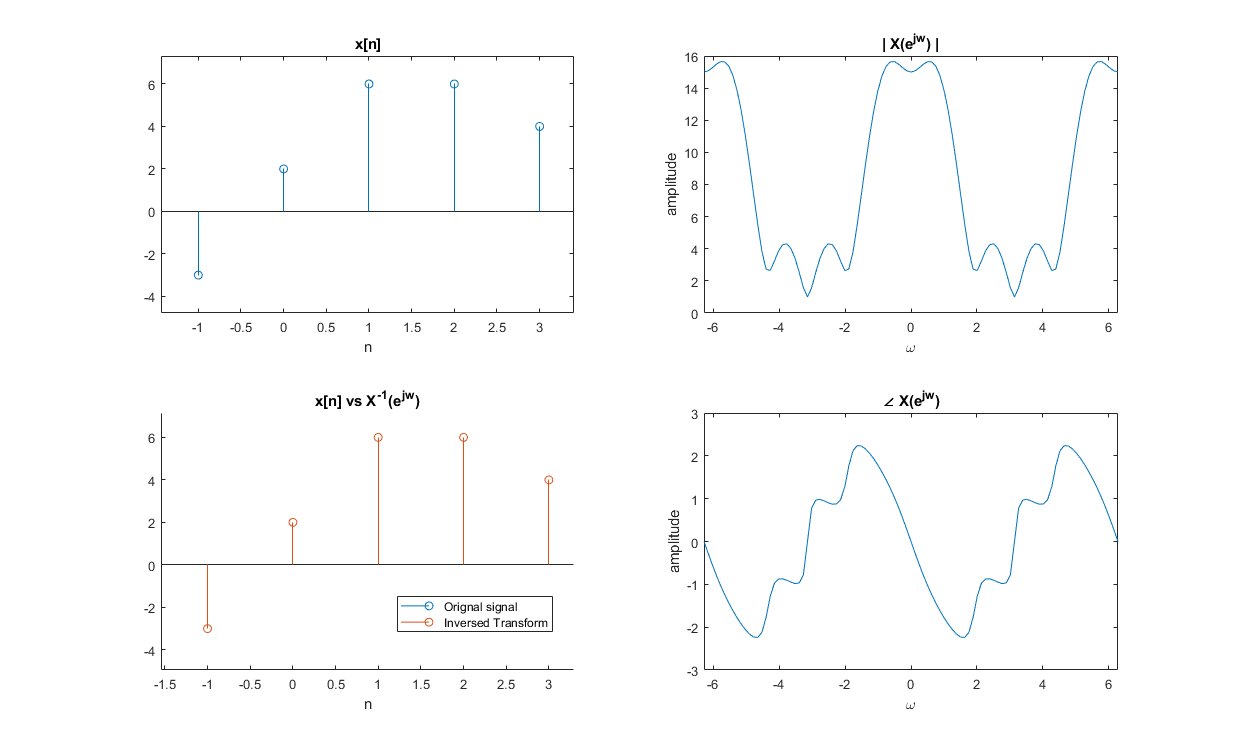
\includegraphics[width=\textwidth]{q1_n=100}
	\caption{DTFT (and Inverse) of x[n]}
\end{figure}
\subsection{q.1b}
A reasonable amount of samples (M) was anything over 100, even then some resolution was lost in the transform. Down at ten all but the largest features of frequency were lost. $X(e^{jw})$ is complex and thus magnitude and phase have been plotted separately (RHS of Fig. 1).

\newpage
\subsection{q.1c}

\begin{figure}[h]
\centering
\begin{subfigure}[b]{.3\linewidth}
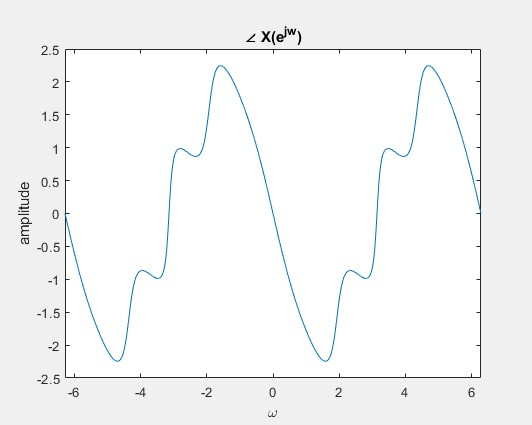
\includegraphics[width=\linewidth]{secondabout0}
\caption{shift by 1}
\end{subfigure}
\begin{subfigure}[b]{.3\linewidth}
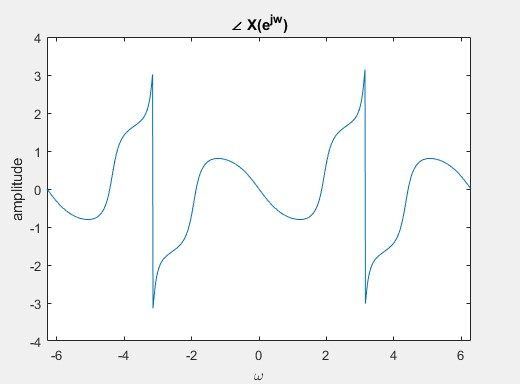
\includegraphics[width=\linewidth]{thirdabout0}
\caption{shift by 2}
\end{subfigure}
\begin{subfigure}[b]{.3\linewidth}
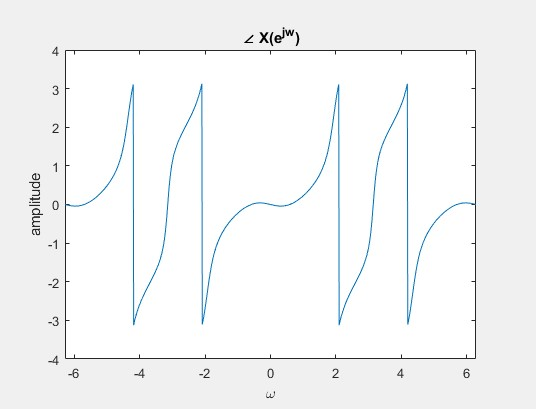
\includegraphics[width=\linewidth]{forthabout0}
\caption{shift by 3}
\end{subfigure}\caption{x[n] shifted by different integer values}
\end{figure}

As x[n] has been shifted in 'n' the transforms gets corresponding phase change.
$$x[n - N_{0}] \Rightarrow e^{-j\omega N_{0}}X(j\omega)$$
As Figure 2 shows as x is shifted at different $N_{0}$ the phase of $X(j\omega)$ changes correspondingly.
\\ \\
\section{Inverse DTFT}
\subsection{q.2b}
As seen Fig 1 shows (subplot 3), the result of the inverse DTFT overlaid with the original sequence shows no difference.\\
The resulting sequence does have complex components but these are not significant as they are all real part + 0j. This is probably due to the transform vector being of complex doubles and MATLAB's matrix operation hence result in a complex vector sequence.

\newpage
\section{Filtering}
\subsection{q.3a}
\begin{figure}[h]
	\begin{center}
	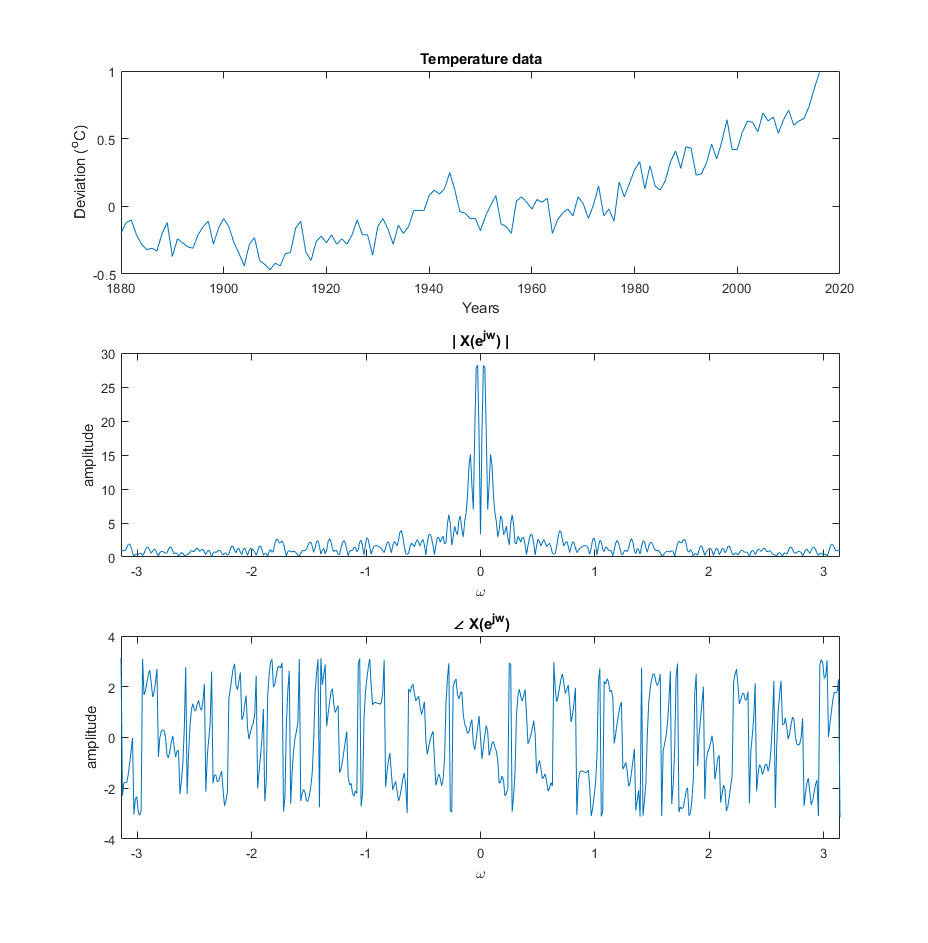
\includegraphics[width=.5\textwidth]{q3_data}
	\caption{Imported Temperature Data and Transform}
	\end{center}
\end{figure}

Figure 3 above shows show the plotted Temperature data and the Mag/Phase plots of this transform. As shown the data has highly contributing low frequency and lots of smaller contributing high frequency oscillations.
\subsection{q.3b}
\begin{figure}[h]
	\begin{center}
	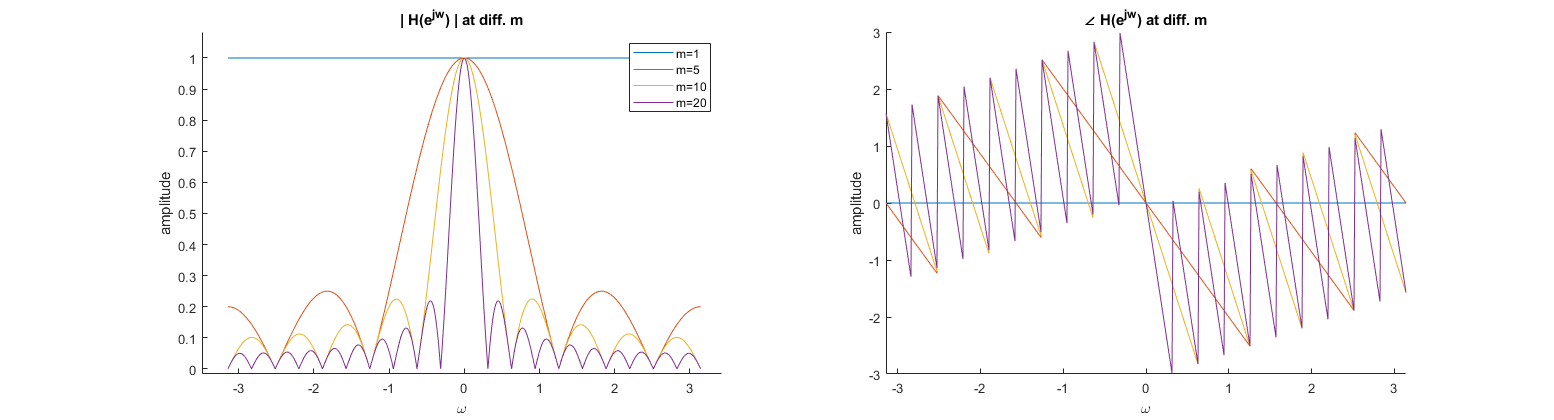
\includegraphics[width=0.8\textwidth]{q3_H}
	\caption{$H(e^{j\omega}$, moving-average filter at diff. m)}
	\end{center}
\end{figure}
Fig. 4 Above is the plotted Mag/Phase of the moving average filter implementation. As seen the increasing m value narrows the high amplitude bandwidth in $\omega$.

\newpage
\subsection{q.3c}
\begin{figure}[h]
	\begin{center}
	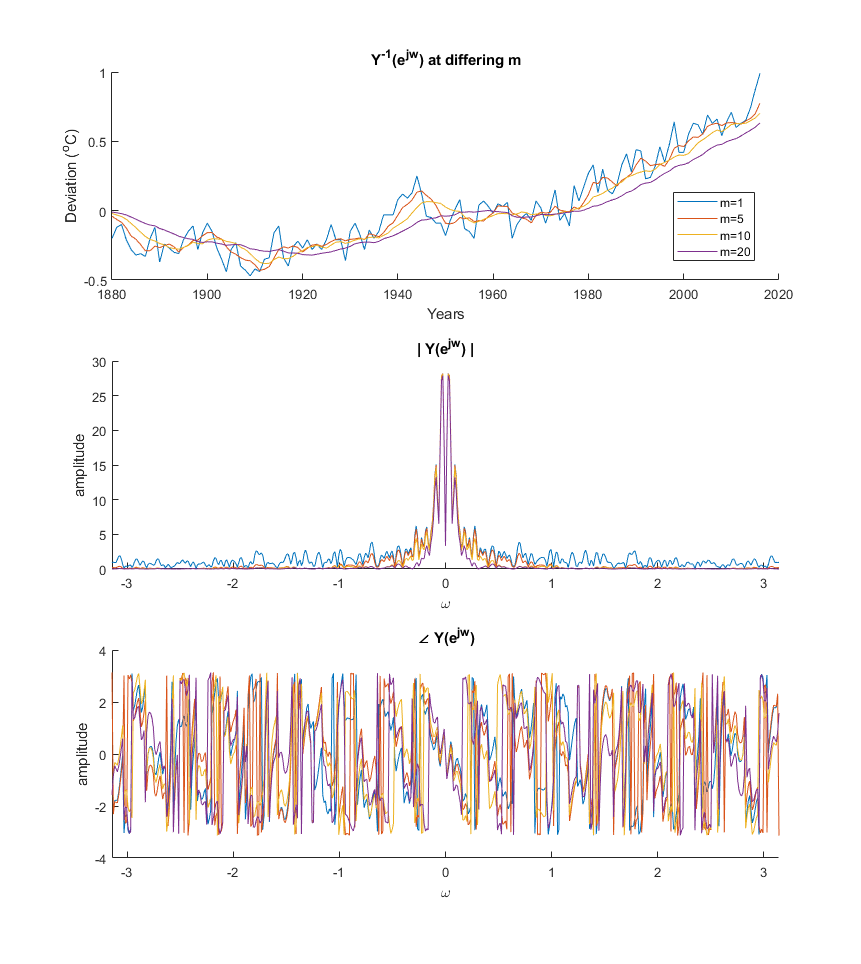
\includegraphics[width=0.7\textwidth]{q3_filtered}
	\caption{Filter applied to data signal at diff. m}
	\end{center}
\end{figure}

The moving-average acts as  a low pass filter with its cutoff determined by m. As Fig. 5 shows m=1 is an unmodified signal (see Fig 4, m=1 $|H(e^{j\omega})|$ = 1, $\angle H(e^{j\omega})$ = 0) and as m increases the filtered signal is low pass filtered to a greater and greater extent. As previously shown $H(e^{j\omega})$  "sharpens" around 0 as m increases and this increases the strength of the low pass filtering.


%----------------------------------------------------------------------------------------
%	APPENDIX
%----------------------------------------------------------------------------------------
\newpage
\section*{Appendix}

\subsection*{DTFT}
\lstinputlisting[language=Matlab]{dtft.m}
\subsection*{Inverse DTFT}
\lstinputlisting[language=Matlab]{invdtft.m}
\subsection*{Q1 / Q2}
\lstinputlisting[language=Matlab]{lab4_12.m}
\newpage
\subsubsection*{Q3}
\lstinputlisting[language=Matlab]{lab4_3.m}

\end{document}
